\documentclass[serif]{beamer}

\usepackage[absolute,overlay]{textpos}
\newif\ifQDLE
\QDLEtrue % set to false to desactivate quizz

\ifQDLE\newcommand\QdleTag[3]{%
\begin{textblock*}{30mm}[0,0](3mm,\textheight)
\#QDLE\##1\##2\##3\#
\end{textblock*}}
\else\newcommand\QdleTag[3]{}
\fi


\usetheme{Madrid}


\title{QuizZoodle}
\subtitle{capture your audience!}

\author{J.~Allali}
\institute{QuizZoodle}
\date{}
\logo{%
    
\includegraphics[width=1cm,height=1cm,keepaspectratio]{qdle_100}~%
}
%\setbeamertemplate{items}[square]

\begin{document}

\renewcommand*{\theenumi}{\Alph{enumi}}

\begin{frame}
  \titlepage
\end{frame}

\ifQDLE\begin{frame}
\frametitle{Example of a survey}
\begin{block}{How are you today?}
\begin{enumerate}
\item Excellent
\item Very Good
\item Good
\item Not so Good
\end{enumerate}
\end{block}
\QdleTag{S}{ABCD}{20} % survey, timeout of 20 seconds
\end{frame}
\fi 

\begin{frame}[fragile]
\frametitle{Let's do some maths...}
\begin{block}{Fibonacci numbers}
Fibonacci numbers are the numbers of the following sequence~:\\
$$
0,1,1,2,3,5,8,13,21,\dots
$$
That is $F_0=0$, $F_1=1$ and $F_n = F_{n-1} + F_{n-2}$
\end{block}
\pause
\begin{block}{If $F_i=6765$ and $F_{i+2}=17711$, what is $F_{i+1}$?}
\begin{enumerate}
\item 10935
\item 10946
\item 10966
\end{enumerate}
\only<2>{\QdleTag{Q}{AB*C}{}} % question, default timeout
\end{block}
\end{frame}

\begin{frame}[fragile]
\frametitle{Just for fun!}
\begin{figure}
   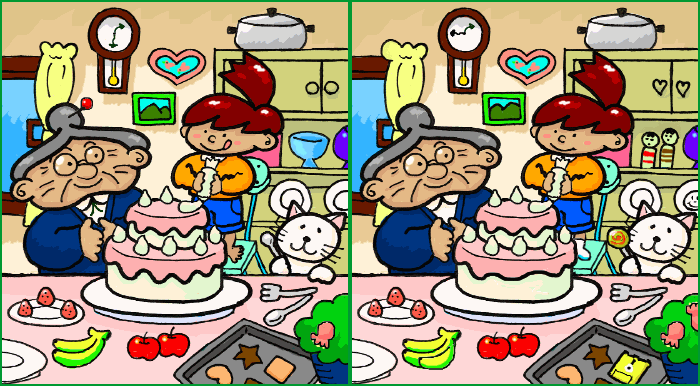
\includegraphics[width= 0.8\linewidth]{Spot_the_difference.png}
   \caption{source: wikipedia, author: Muband}
\end{figure}
How many errors? $A\Rightarrow 7$ ;  $B \Rightarrow 10$ ; $C \Rightarrow 15$
\QdleTag{Q}{ABC*}{120}
\end{frame}

\begin{frame}[fragile]
\frametitle{QdleTag how to}
\begin{itemize}
\item Including QuizZoodle into your presentation is really easy.
\item Just design your slides and include a tag into slides that contain
quizz or survey.
\end{itemize}
\pause
\begin{block}{quizzoodle tags}
The regular expression for tag is the following~:\\
\#QDLE\#(Q$|$ S)\#[ABCD*]+\#([0-9]+\#)?\\
That is:
\begin{enumerate}[1]
\item start with \#QDLE\#
\item if its a question Q\# followed by the set of possible answers (ABCD), the right one must be followed by a *
\item if its a survey S\# followed by the set of possible answers (ABCD)
\item optionally a specific timeout (if not set, the global quizz timeout will be used).
\end{enumerate}
\end{block}
\end{frame}

\begin{frame}[fragile]
\frametitle{QdleTag how to (2)}
\begin{itemize}
\item You will find at the beginning of the source of this presentation a \LaTeX macro that will ease the inclusion of tags without disrupting your slide layout.
\item Sometime, they can be error in pdf rendering, try to re-encode your pdf using the command: \verb+ pdf2ps slides.pdf - | ps2pdf - out.pdf +
\item Hope you enjoy QuizZoodle and will use it very soon!
\end{itemize}
\pause
\begin{block}{How you find the presentation?}
\begin{enumerate}
\item awesome
\item very cool
\item nice
\item useless
\end{enumerate}
\only<2>{\QdleTag{S}{ABCD}{45}}
\end{block}
\end{frame}



\end{document}
